\section{Embedding into Sierpinski Tetrahedron}

\begin{frame}
	\frametitle{Constraction of Sierpinski Tetrahedron\cite{Quanta}}
	\begin{figure}[!htb]
		\begin{minipage}{0.5\textwidth}
			\centering
			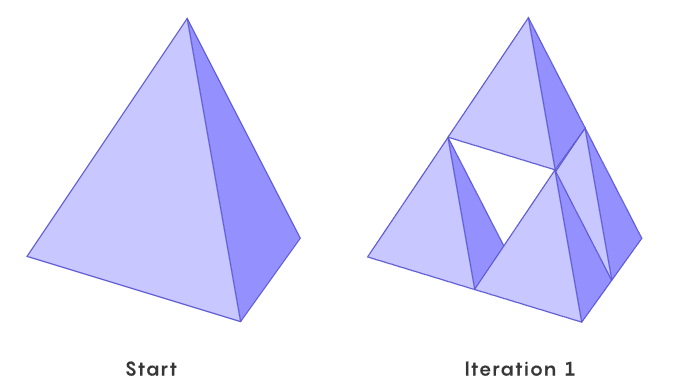
\includegraphics[width=1.0\linewidth]{images/SierpinskiTet}
		\end{minipage}\hfill
		\begin{minipage}{0.5\textwidth}
			\centering
			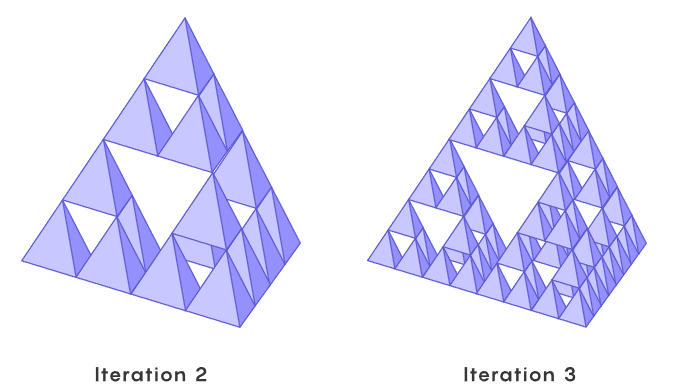
\includegraphics[width=1.0\linewidth]{images/SierpinskiTet2}
		\end{minipage}
	\end{figure}
	\begin{itemize}
		\item Similar construction like the construction of the Menger Sponge.
		\item Each face is an iteration of the Sierpinski Triangle.
	\end{itemize}
\end{frame}

\begin{frame}
	\frametitle{Difficulties}
	\begin{center}
	\begin{tabular}{|c|c|}
		\hline
		\textbf{Menger Sponge} & \textbf{Sierpinski Tetrahedron} \\
		\hline
		Easily understandable representation  & Difficulties caused by tetrahedrons \\
		\hline
		arc representation & ? \\
		\hline
	\end{tabular}
	\end{center}\\
	\\
	\onslide<2->
	Solution:
	\begin{itemize}
		\item Combinatorial representation of the Sierpinski Tetrahedron
		\item Pretzel knots
	\end{itemize}
\end{frame}

\begin{frame}
	\frametitle{Combinatorial representation of the Tetrahedron} % Changed from "Frame-titel"
	\begin{figure}[h]
		\centering
		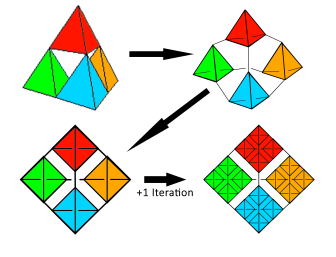
\includegraphics[width=0.5\linewidth]{images/CombRep1}
		\caption{Combinatorial representation of the Tetrahedron \cite{broden2024knotsinsidefractals}}
		\label{fig:enter-label}
	\end{figure}
\end{frame}

\begin{frame}
	\frametitle{Combinatorial representation of the Tetrahedron} % Changed from "Frame-titel"
	\begin{figure}[h]
		\centering
		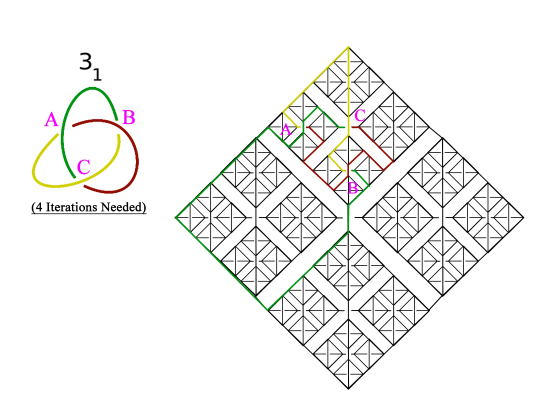
\includegraphics[width=0.5\linewidth]{images/CombRep2}
		\caption{Example $3^1$ knot \cite{broden2024knotsinsidefractals}}
		\label{fig:enter-label}
	\end{figure}
\end{frame}

\begin{frame}
	\frametitle{Combinatorial representation of the Tetrahedron} % Changed from "Frame-titel"
	\begin{figure}[h]
		\centering
		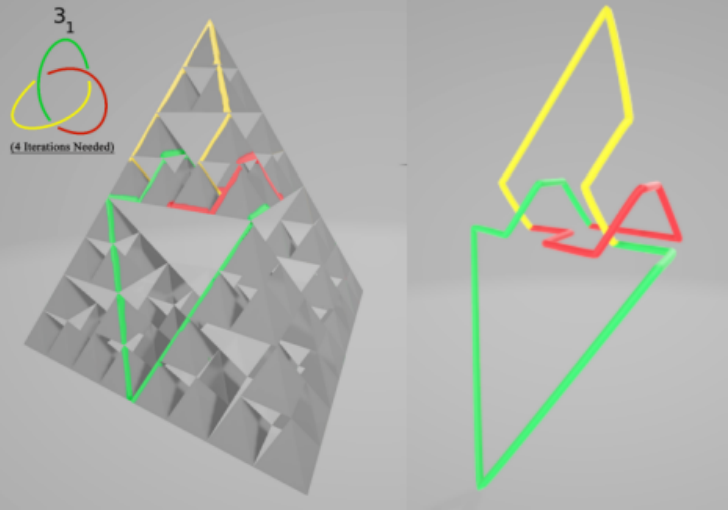
\includegraphics[width=0.5\linewidth]{images/CombRep3}
		\caption{Example $3^1$ knot \cite{broden2024knotsinsidefractals}}
		\label{fig:enter-label}
	\end{figure}
\end{frame}

\begin{frame}
	\frametitle{Sierpinski Tetrahedron} % Changed from "Frame-titel"
	\begin{theorem}
		All Pretzel Knots are inside a finite iteration of the Sierpinski Tetrahedron. \cite{broden2024knotsinsidefractals}
	\end{theorem}
	\onslide<2->
	\begin{proof}
		\begin{lemma}
			Every isolated helix can be put inside a finite iteration of the tetrahedron. \cite{broden2024knotsinsidefractals}
		\end{lemma}
		\onslide<3->
		To finish the proof they showed, that the helices can be connected as required.  
	\end{proof}
	\onslide<4->
	\begin{itemize}
		\item It is easy to follow that a certain Pretzel knot in which iteration can be embedded.
	\end{itemize}
\end{frame}

\begin{frame}
	\frametitle{Sierpinski Tetrahedron}
	\begin{figure}[h]
		\centering
		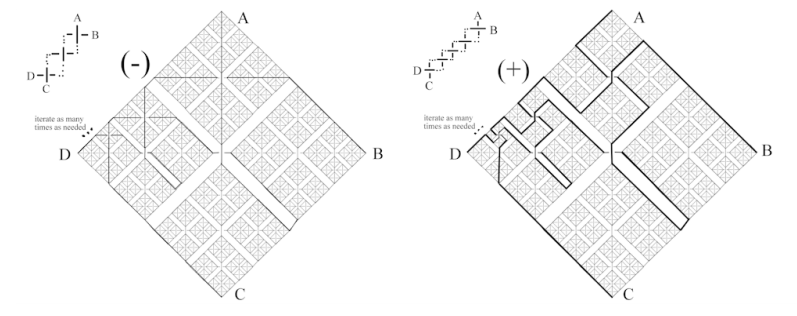
\includegraphics[width=1.0\linewidth]{images/Helix1}
		\caption{Helices in a certain iteration. \cite{broden2024knotsinsidefractals}}\label{Fig:Helix1}
	\end{figure}
\end{frame}

\begin{frame}
	\frametitle{Sierpinski Tetrahedron}
	\begin{figure}[!htb]
		\begin{minipage}{0.4\textwidth}
			\centering
			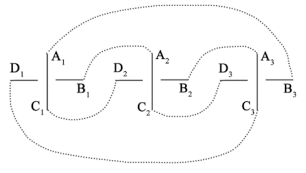
\includegraphics[width=1.0\linewidth]{images/SimplifiedPretzelKnot}
			\caption{Every Pretzel Knot can be simplified to the above form. \cite{broden2024knotsinsidefractals}}\label{Fig:SimplifiedPretzelKnot}
		\end{minipage}\hfill
		\begin{minipage}{0.6\textwidth}
			\centering
			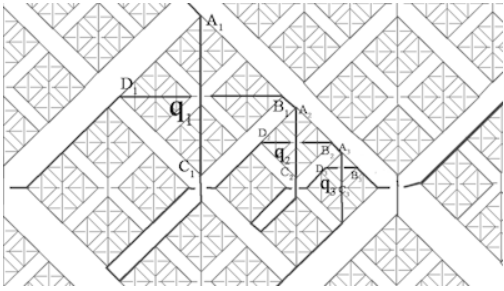
\includegraphics[width=1.0\linewidth]{images/ConnectHelices}
			\caption{It is possible to connect the helices in the required order. \cite{broden2024knotsinsidefractals}}\label{Fig:ConnectHelices}
		\end{minipage}
	\end{figure}
\end{frame}

\begin{frame}
	\frametitle{Comparison between Fractals} % Changed from "Frame-titel"
	Denote with $M_n$ and $S_n$ the one-skeleton of the $n^{th}$ iteration of the Menger sponge and the Sierpinski Tetrahedron.\\
	Let $M(K)=\min{n}$, such that $K\subset M_n$. Similarly $S(K)=\min{n}, s.t. K\subset S_n$.\\
	\onslide<2->
	\begin{theorem}
		Let K be a not, then we have
		$$M(K)\leq S(K),$$
		whenever $S(K)$ is defined. \cite{broden2024knotsinsidefractals}
	\end{theorem}
	
	\onslide<3->
	\begin{proof}
		Shortly: The one-skeleton of the $i^{th}$ iteration of the Sierpinski Tetrahedron can be embedded into the one-skeleton of the $i^{th}$ iteration of the Menger Sponge. This embedding preserves the knot type.
	\end{proof}
\end{frame}

\begin{frame}
	\frametitle{Comparison between Fractals} % Changed from "Frame-titel"
	\begin{figure}[!htb]
		\begin{minipage}{0.48\textwidth}
			\centering
			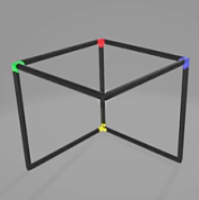
\includegraphics[width=0.42\linewidth]{images/Comparison1}
			\caption{$S_0$ in $M_0$ \cite{broden2024knotsinsidefractals}}\label{Fig:Data1}
		\end{minipage}\hfill
		\begin{minipage}{0.48\textwidth}
			\centering
			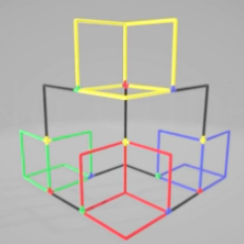
\includegraphics[width=0.42\linewidth]{images/Comparison2}
			\caption{$S_1$ in $M_1$ \cite{broden2024knotsinsidefractals}}\label{Fig:Data2}
		\end{minipage}
	\end{figure}
	\onslide<2->
	What next?
	\onslide<3->
	\begin{itemize}
		\item To get $S_2$ in $M_2$: replace every $S_0$ in $S_1$ by $S_1.$
		\onslide<4->
		\item To get $S_{n+1}$ in $M_{n+1}$: replace every $S_0$ in $S_n$ by $S_1.$
		\onslide<5->
		\item Substitutions are in disjoint regions, so the embedding preserves the knot type.
	\end{itemize}
\end{frame}

\begin{frame}
	\frametitle{Open questions \cite{broden2024knotsinsidefractals}}
	\begin{itemize}
		\item Every knot can be embedded into the Sierpinski tetrahedron.
		\onslide<2->
		\begin{figure}[h]
			\centering
			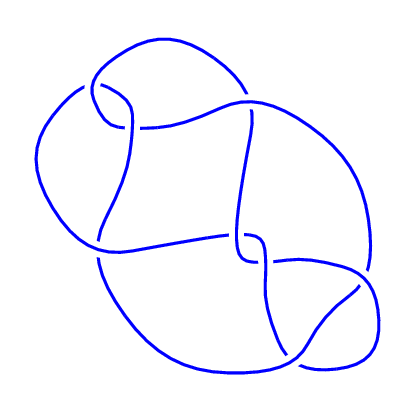
\includegraphics[width=0.25\linewidth]{images/8_12}
			\caption{$8_{12}$ knot is not a Pretzel knot \cite{knotinfo}}\label{Fig:8_12}
		\end{figure}
		\onslide<3->
		\item Is there a fractal defined by iterative steps that doesn't admit all of the knots? If it is so, what does this tell us about the fractal?
	\end{itemize}
\end{frame}